\section{The CMS and Tau Reconstruction}
\begin{frame}{CMS Detector}
    \begin{center}
        \includegraphics[width=0.9\textwidth]{chapters/CMSExperiment/sectionDetector/figures/cmsDetector.png}
    \end{center}
\end{frame}



%

\begin{frame}{}
\smaller
    \begin{columns}
    \column{0.6\textwidth}

    \begin{itemize} 
        \item Brain of the detector: Two-level trigger system.
        \item level-1 trigger (L1T)
        \begin{itemize} 
            \item customized ASICs and onsite FPGAs
            \item consider muon chamber and calorimeter
            \item 40MHz to 100kHz
            \item comprised of local, regional and global 
            \item latency budget 4\mus 
        \end{itemize}
        
        \item high-level trigger (HLT)
        \begin{itemize} 
            \item CPU. commodity computers of builder-filter.
            \item run a streamlined version of offline reconstruction software, filter with a HLT menu
            \item 100\;kHz to 1\;kHz
            \item in 2012, 13000 CPU cores 200 ms/event \cite{Trocino:2014jya}
        \end{itemize}
    \end{itemize}
    
    
    \column{0.4\textwidth}
    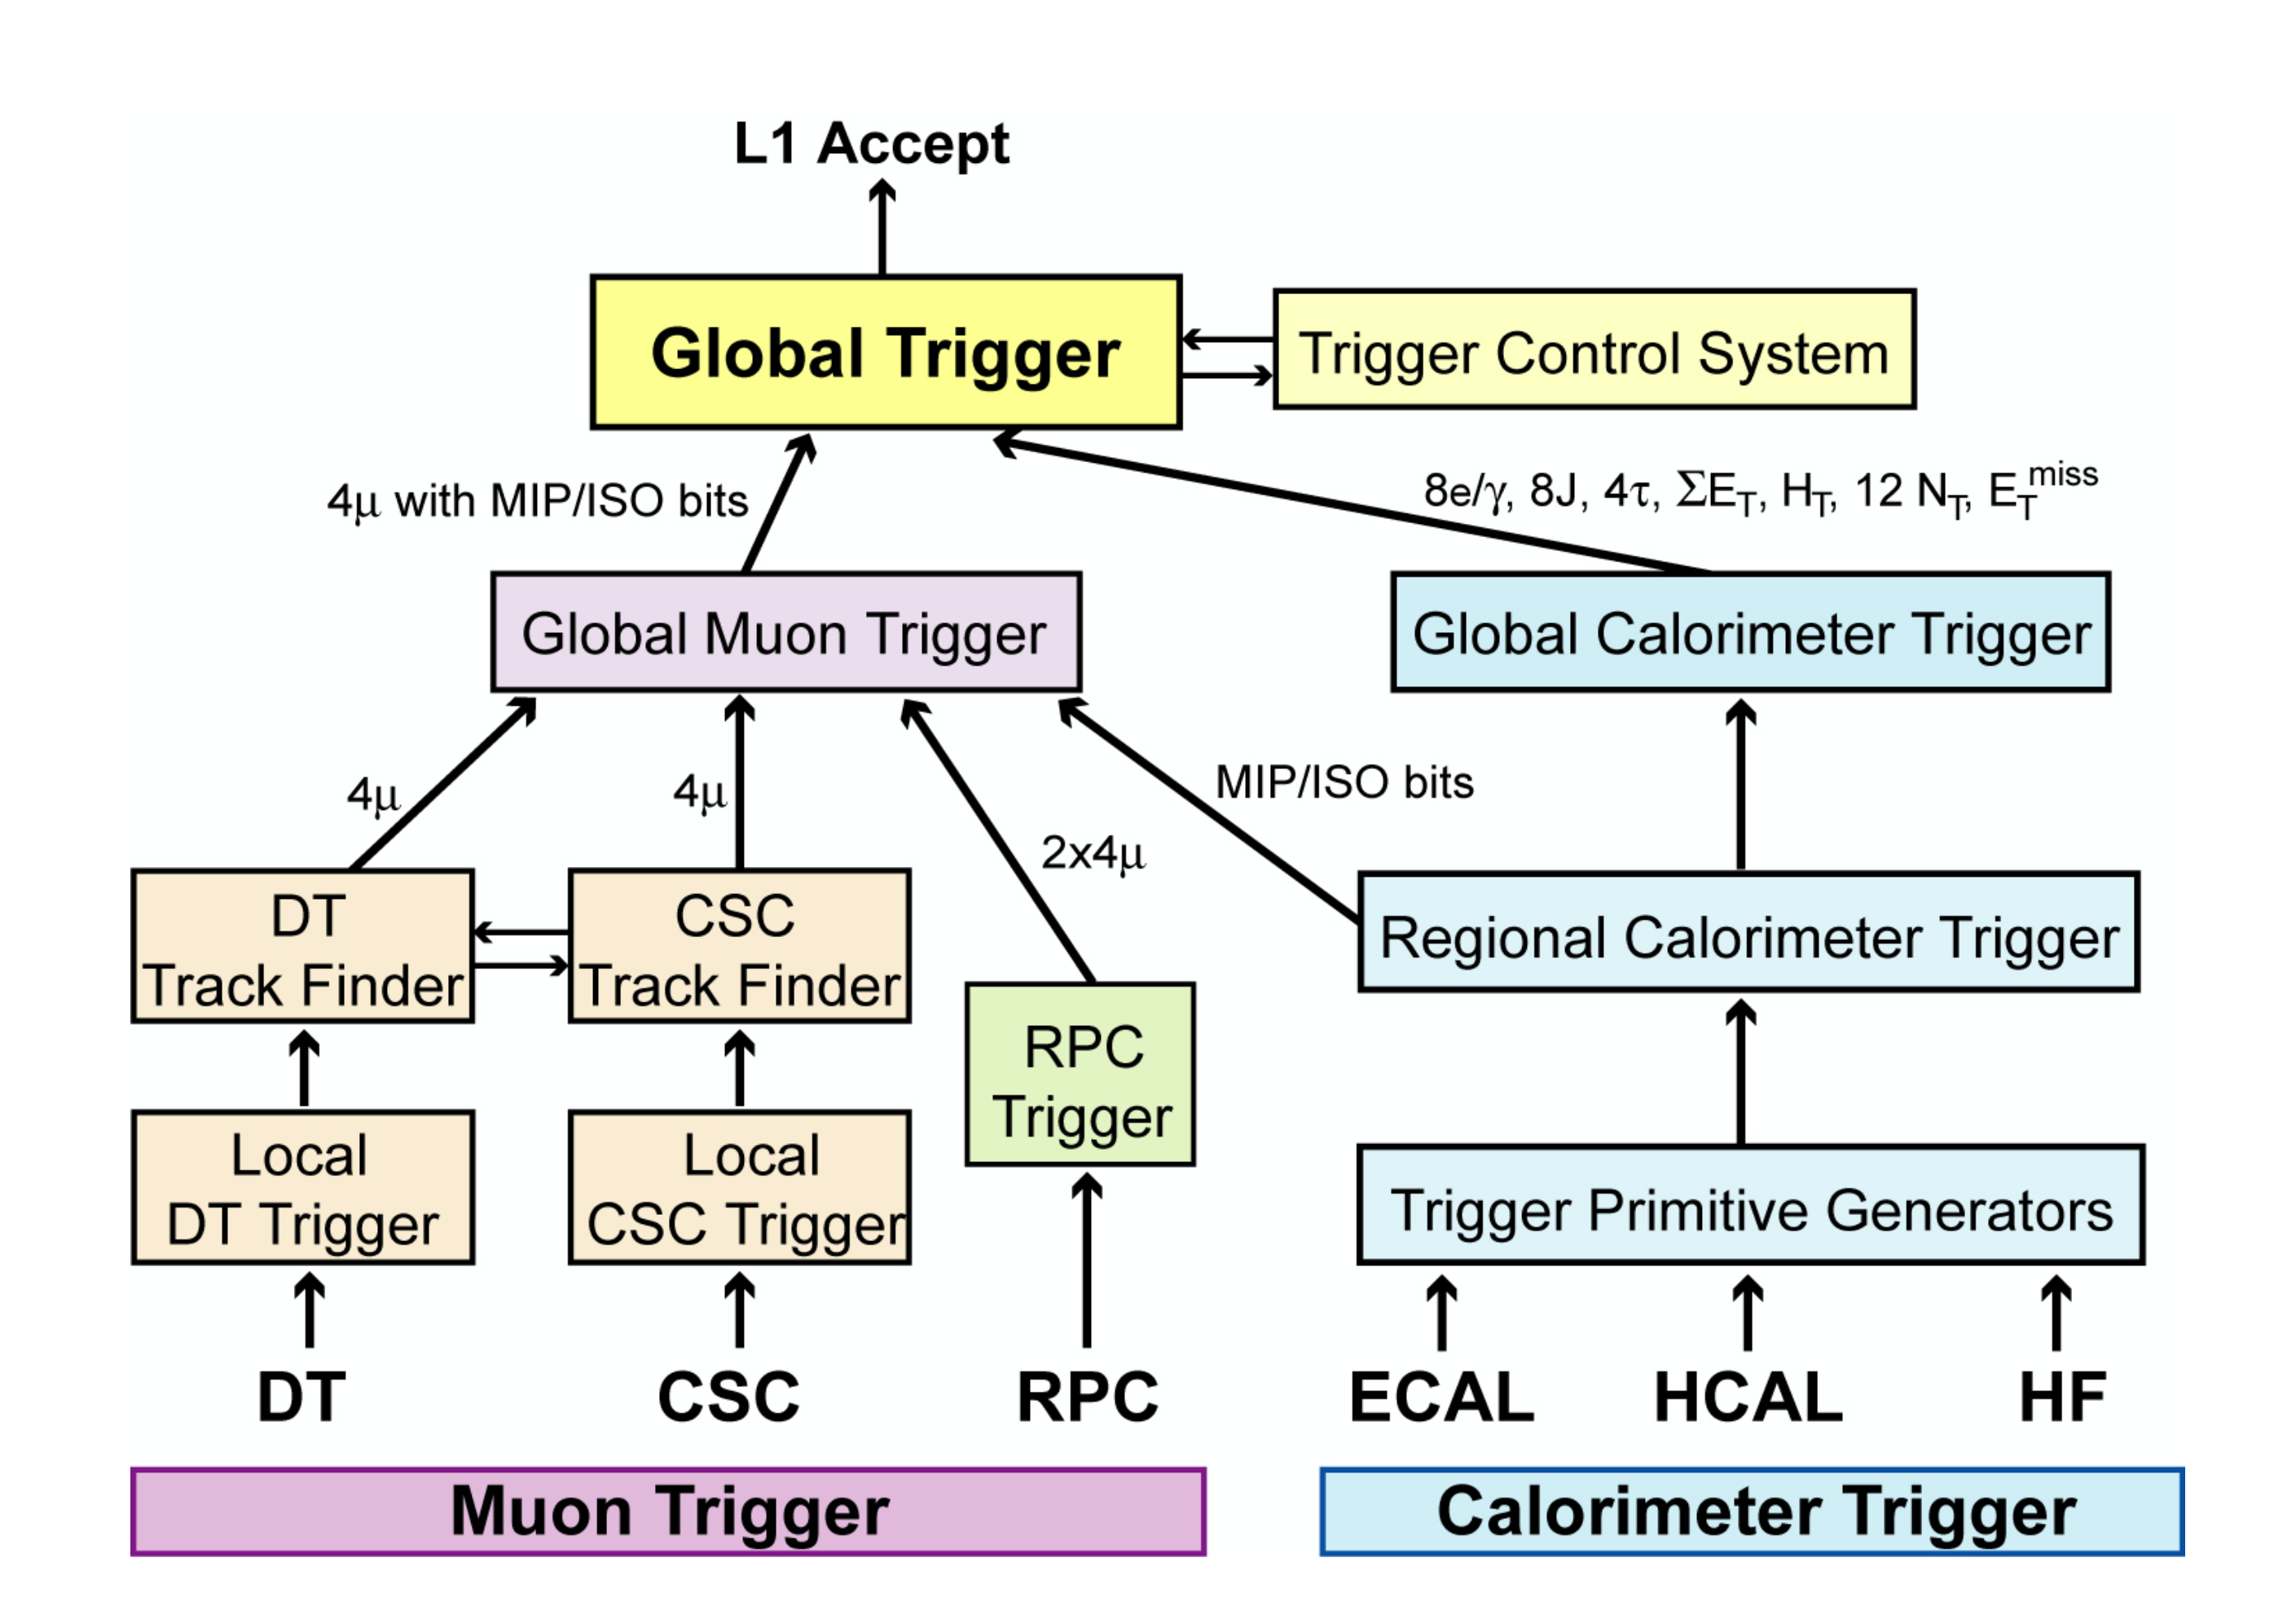
\includegraphics[width=\textwidth]{chapters/CMSExperiment/sectionTrigger/figures/trigger.png}
    \end{columns}
\end{frame}


\begin{frame}{CMS Detector}
    \begin{center}
        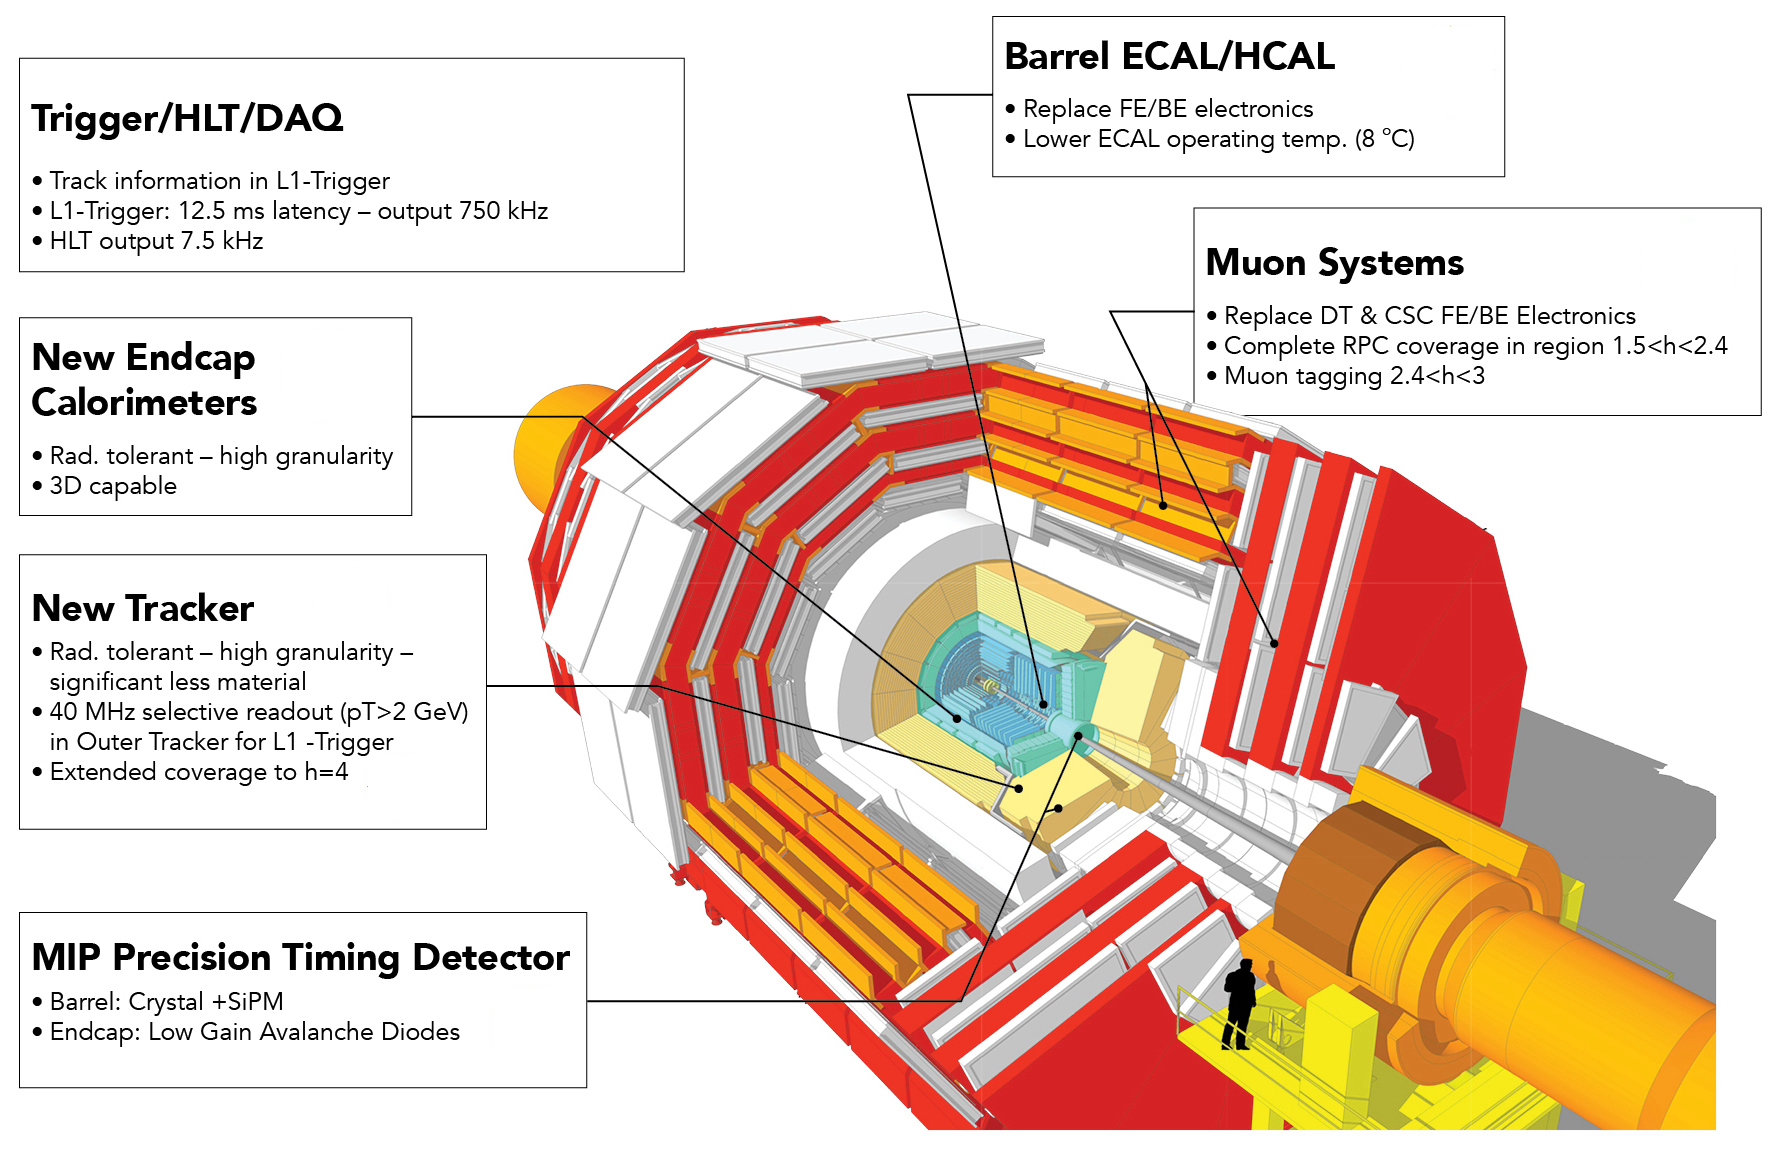
\includegraphics[width=0.9\textwidth]{slides/figures/CMS_NSF_DOE.jpeg}
    \end{center}
    \footnote{ https://www.classe.cornell.edu/NewsAndEvents/CLASSENewsCMS180129Ryan.html}
\end{frame}




\begin{frame}{Particle-Flow Reconstruction}
\smaller
    \begin{center}
        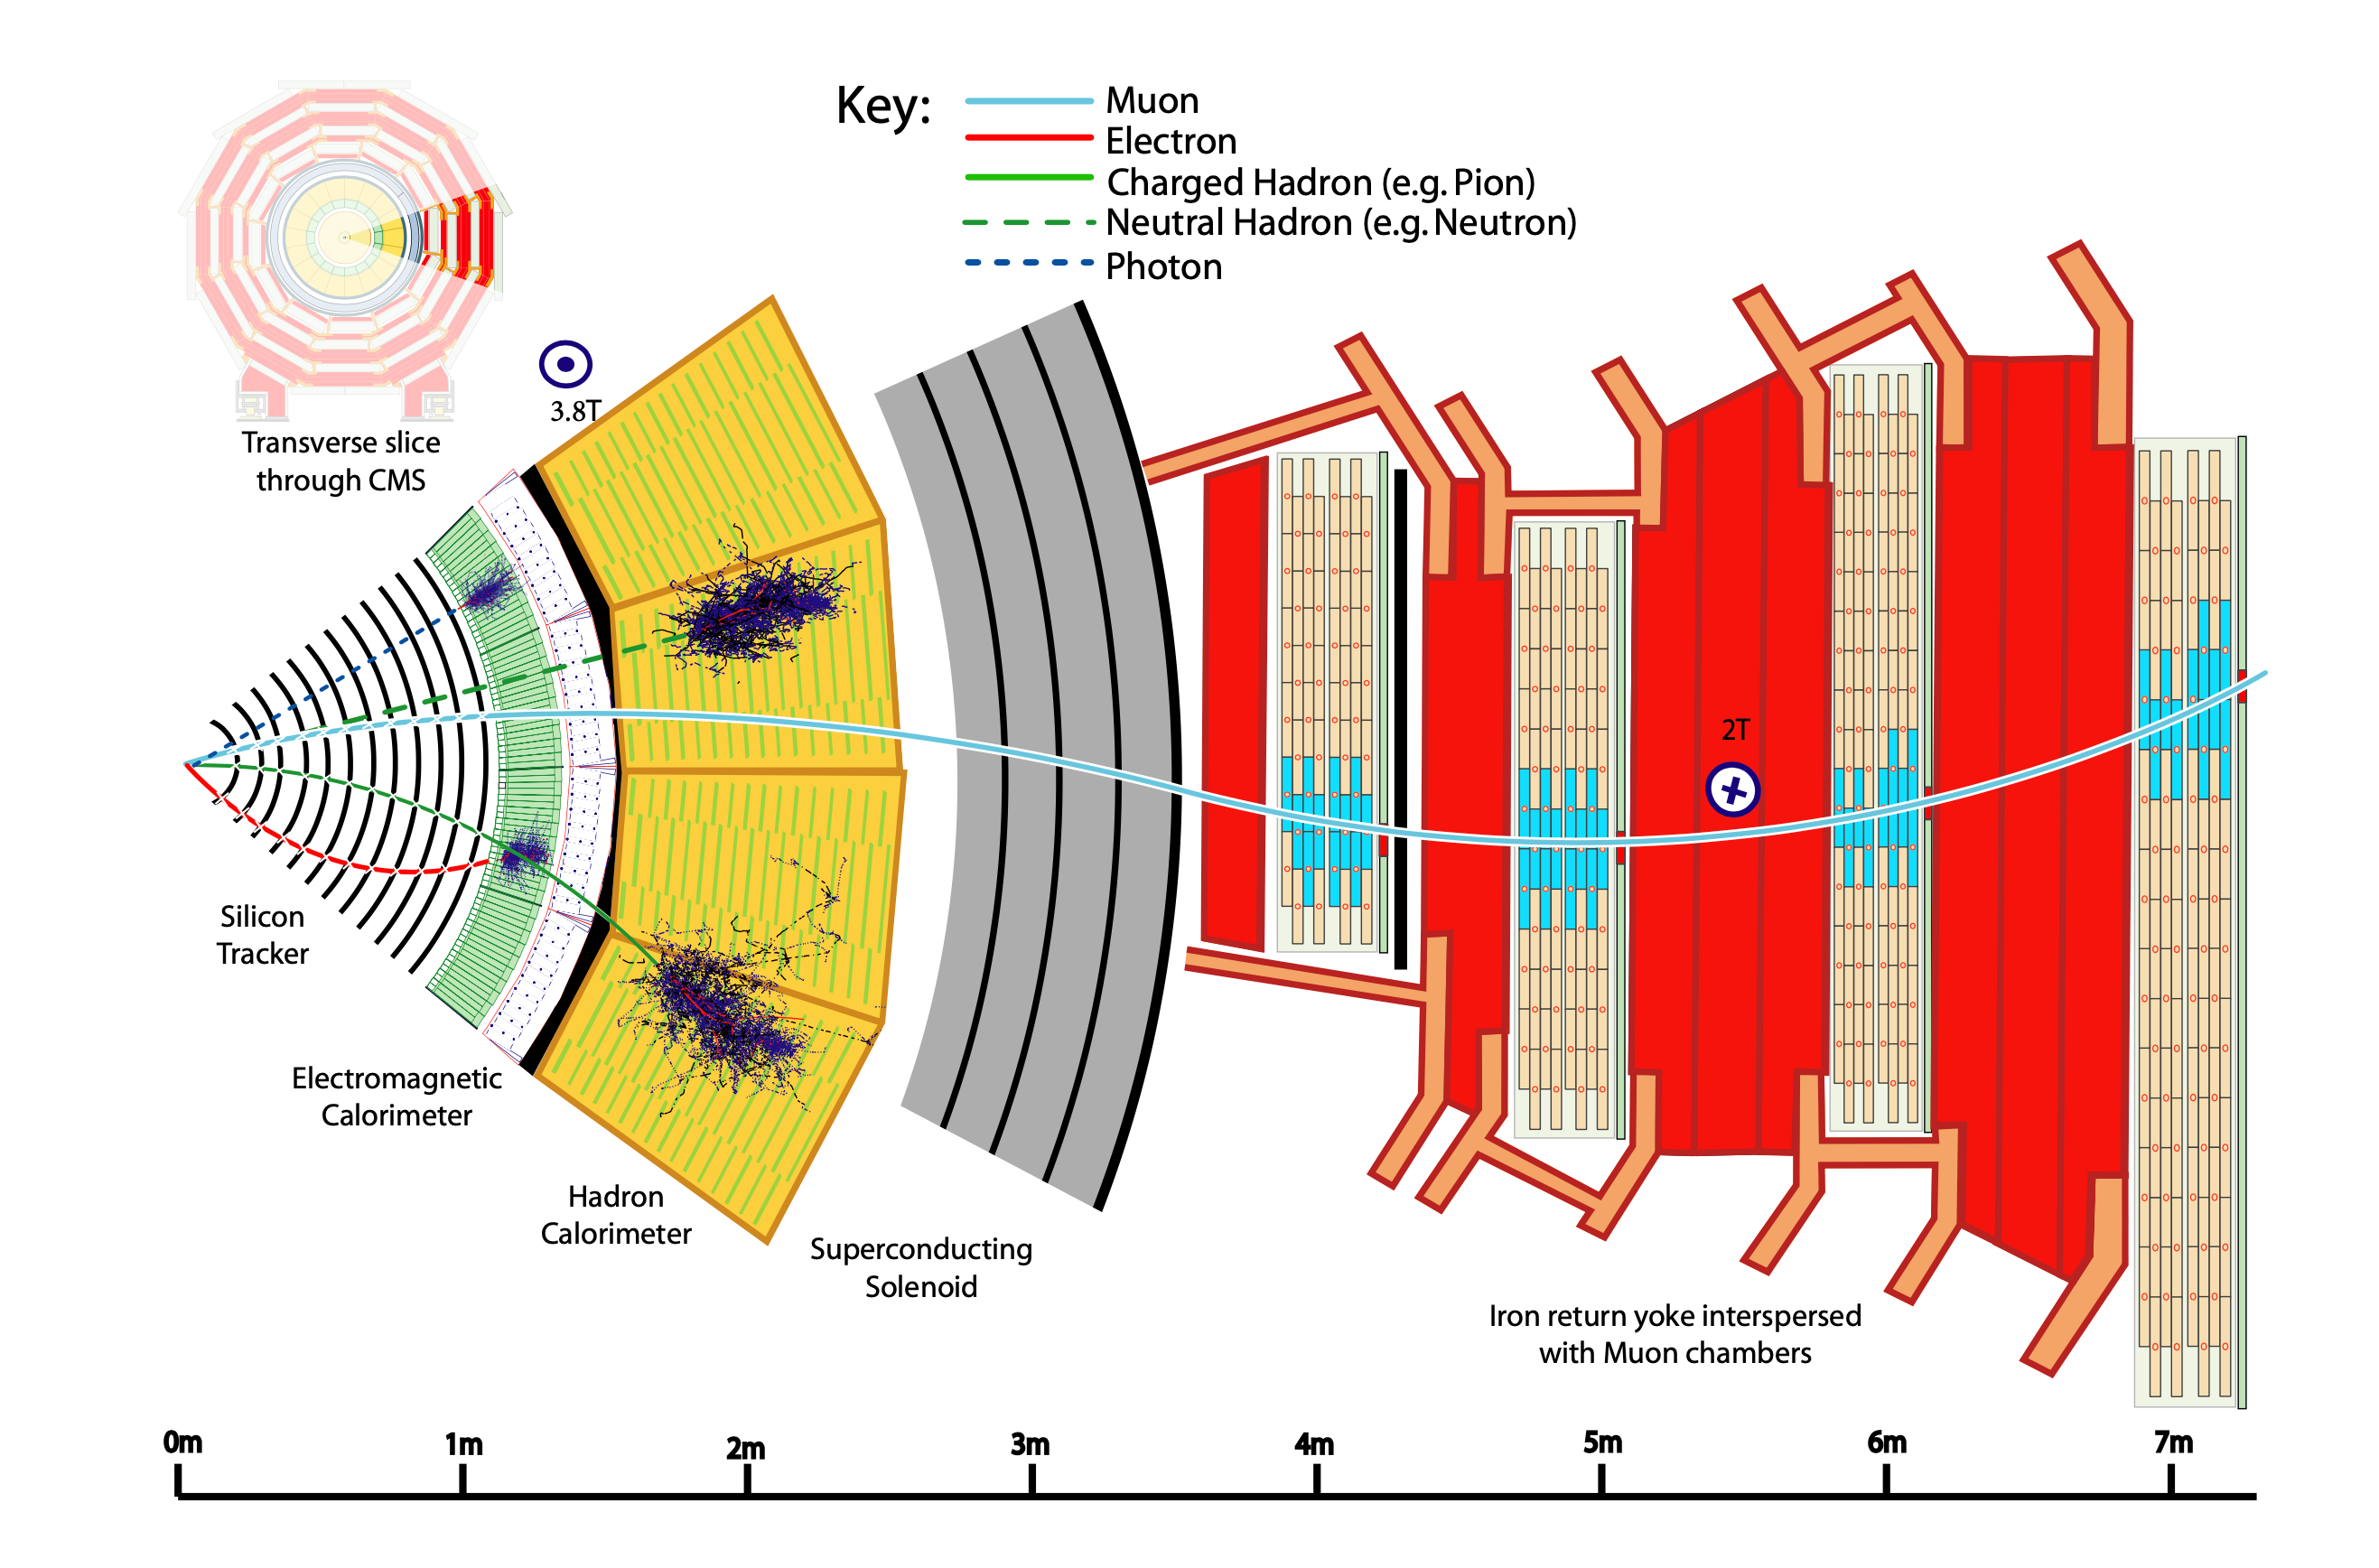
\includegraphics[width=0.7\textwidth]{chapters/CMSExperiment/sectionReconstruction/figures/pfa.png}
    \end{center}
    \begin{itemize} 
        \item combines information in all subdetector to construct final state particles (called PF candidate) muon, electron, charged hadron, neutral hadron, photon.
        \item main steps PF blocks, linking, identification/energy regression.
        \item Jets are clustered by anti-\kt based on PF candidates. 
    \end{itemize}
\end{frame}

\begin{frame}{Hadronic Tau Reconstruction}
\smaller
    \begin{center}
        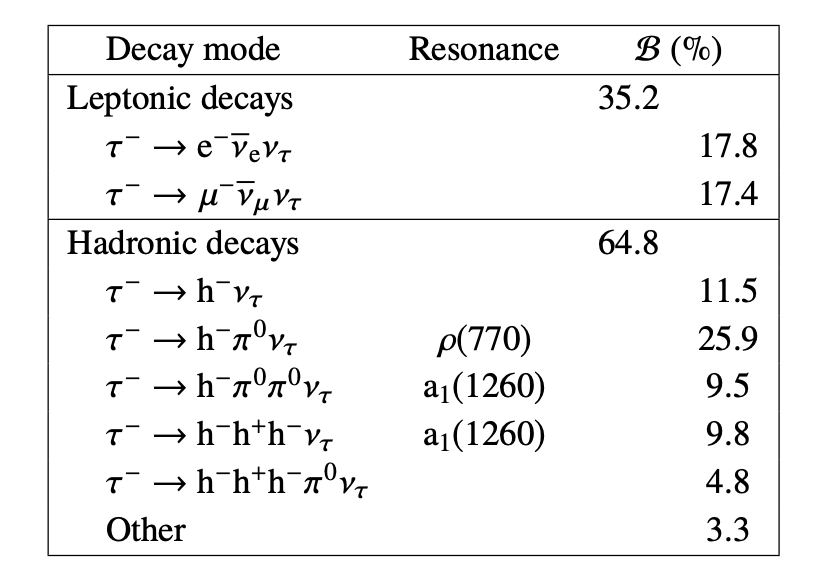
\includegraphics[width=0.5\textwidth]{slides/figures/tauDecay.png}
    \end{center}
    \begin{block}{Tau Property}
    \begin{itemize} 
        \item mass $m_\PGt = 1.776\GeV$ and lifetime $c\Gamma = 87\mum$
        \item 65\% decay hadronically
        \item fixed pattern of final-state particles
        \item defined visible mass at $\rho (770)$ and $a_1(1260)$
    \end{itemize}  
    \end{block}
\end{frame}

\begin{frame}{}
\smaller
    \begin{center}
        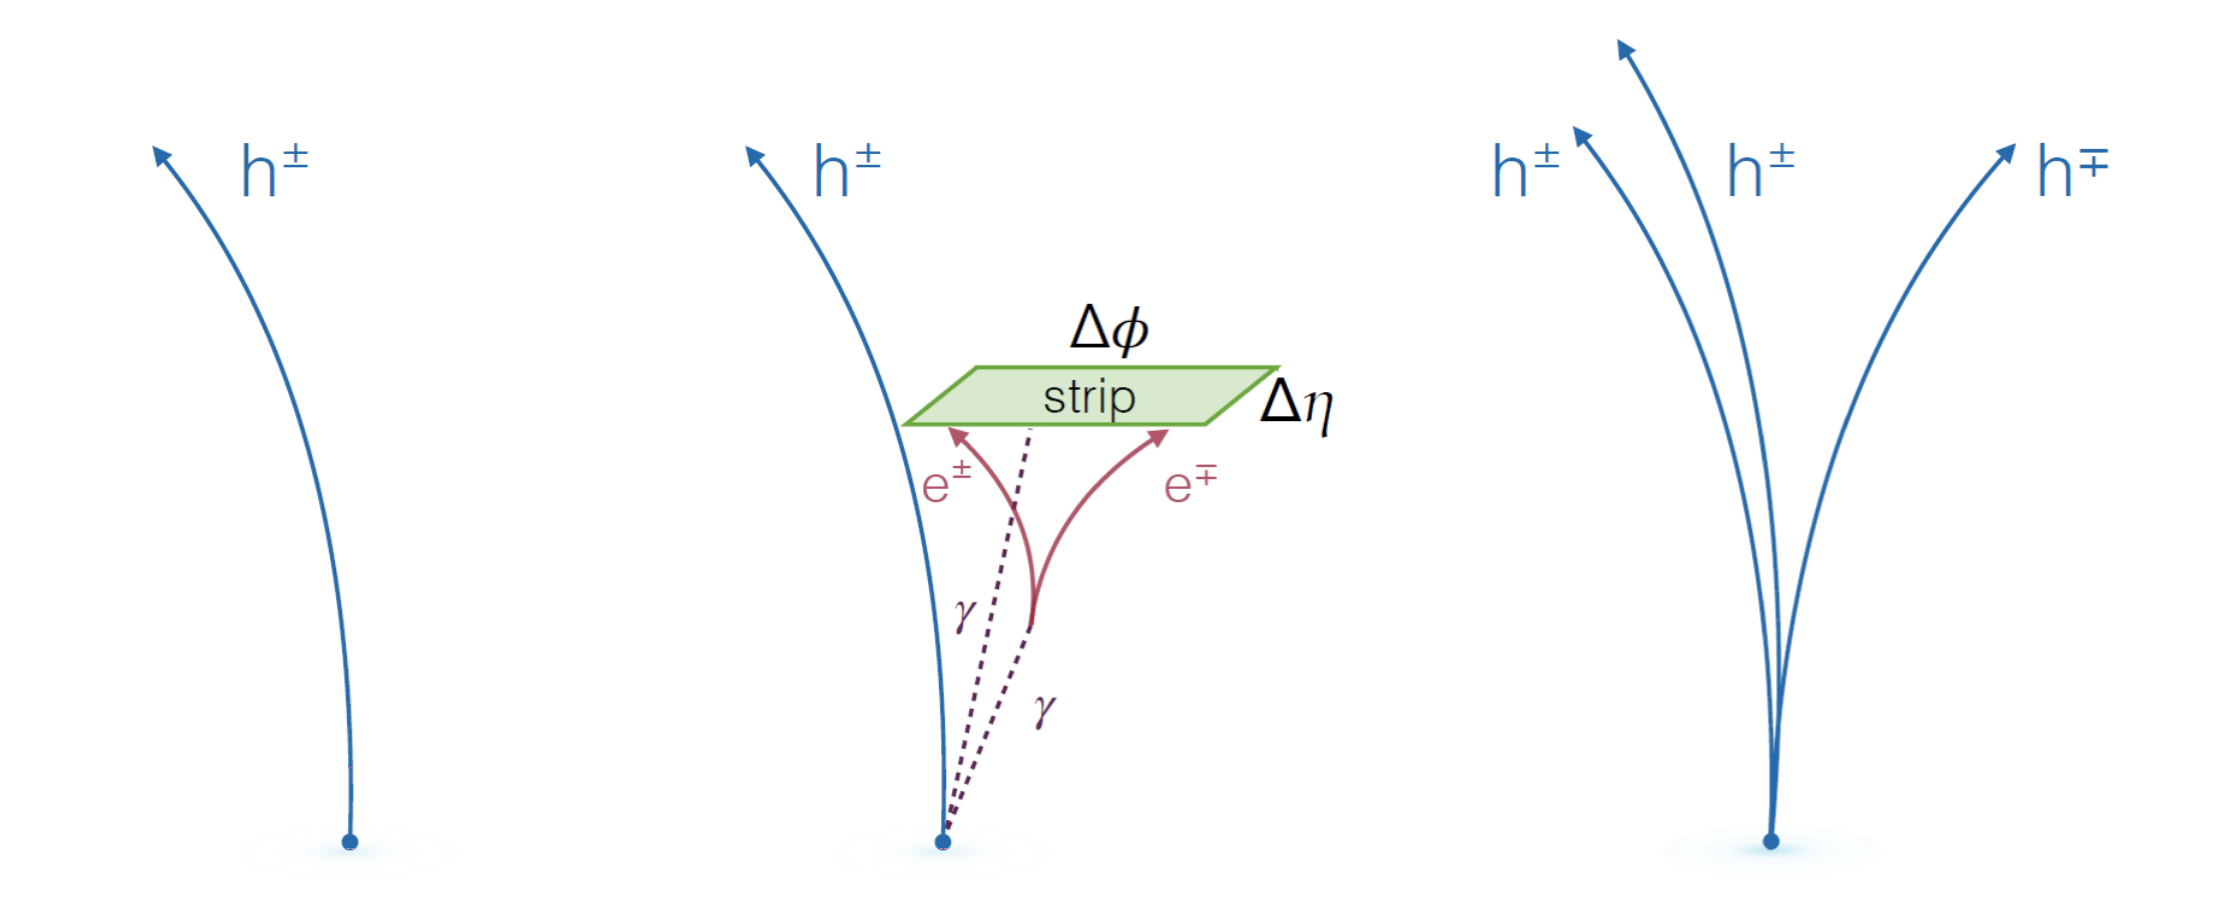
\includegraphics[width=0.6\textwidth]{slides/figures/tauReco.png}
    \end{center}
    \begin{block}{Hadrons-plus-strips (HPS)}
    Taus are reconstructed in their hadronic modes with Hadrons-plus-strips (HPS) algorithm from tagging PF jets
    \begin{itemize} 
        \item cluster \Pe/\PGg into strips. merging \Pe/\PGg in \pt decreasing order with a dynamic window size $\Delta\eta \times \Delta \phi = 0.20\pt^{-0.66} \times 0.35 \pt^{-0.71}$ 
        \item select charged hadrons (prong) $\pt>0.5\GeV$ and $d_{xy}<0.1$~cm.
        \item match to combination of hadrons and strips to \PGth decay modes.
        \item veto when
        \begin{itemize} 
        \smaller
            \item visible mass not competent with expected $\rho (770)$ and $a_1(1260)$ resonance
            \item not single charged
            \item any component falls outside signal cone $\Delta R_{sig} = \frac{3.0 \text{ GeV } } { \pt (\text{ hadronic system})  }$, with $0.05 \leq \Delta R_{sig} \leq 0.1.$
        \end{itemize}
    \end{itemize}  
    \end{block}
\end{frame}


\begin{frame}{Hadronic Tau Reconstruction}
\smaller
    
    \begin{columns}[c]
        \column{0.6\textwidth}
        \begin{block}{Discriminate against contamination}
        \begin{itemize} 
            \item discriminate against quark and gluon jets.
            \item iso-based discriminator: 
            \begin{itemize} 
            \smaller
                \item isolation is calculated energy sum in the ring between signal cone and $\Delta R = 0.3$ cone.
                \item quark and gluon jets tend to have larger isolation, while tau jets tend to have smaller.
            \end{itemize}
        
             
            % \begin{equation}
            % \tiny
            %     I_{\PGth} = \sum \pt^{\text{charged}} (d_z<0.2 \text{cm}) + \max \bigg( 0, \sum \pt^ \PGg - \Delta \beta \sum \pt^{\text{charged}} (d_z>0.2 \text{cm})  \bigg )
            % \end{equation}
            
            \item MVA-based discriminator: 
            \begin{itemize} 
            \smaller
                \item combine isolation and other variables sensitives to tau lifetime (e.g. SIP3D, d0).
                \item use boosted decision tree (BDT)
            \end{itemize}
        \end{itemize}
        \end{block}

        \column{0.4\textwidth}
        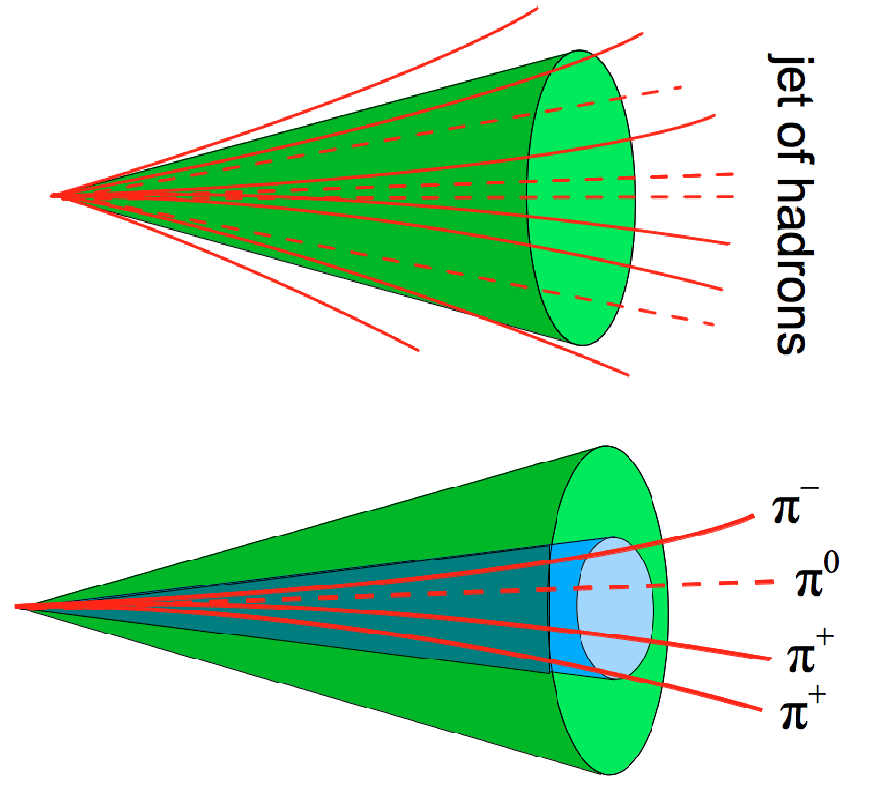
\includegraphics[width=\textwidth]{slides/figures/tausignature_trans.png}
    \end{columns}
    
\end{frame}